\documentclass[../norme-di-progetto.tex]{subfiles}
\begin{document}

\subsection{Gestione organizzativa}
\subsubsection{Scopo}

\subsubsection{Aspettative}

\subsubsection{Descrizione}

\subsubsection{Ruoli}
\paragraph{Responsabile}
\paragraph{Amministratore}
\paragraph{Analista}
\paragraph{Progettista}
\paragraph{Programmatore}
\paragraph{Verificatore}

\subsubsection{Procedure}
\paragraph{Gestione delle comunicazioni}
\subparagraph{Comunicazioni Interne}
\subparagraph{Comunicazioni Esterne}
\paragraph{Gestione degli incontri}
\paragraph{Gestione degli strumenti di coordinamento}
\paragraph{Gestione dei rischi}

\subsubsection{Strumenti}
\paragraph{Visual Studio Code}
Lo sviluppo dell'intero prodotto è eseguito nell'\glossario{IDE} Visual Studio Code, con l'aggiunta delle seguenti estensioni:
\begin{itemize}
  \item \textbf{Git Graph}: permette di utilizzare azioni Git a partire dal grafo della \glossario{repository};
  \item \textbf{LaTeX Workshop}: fornisce tutte le feature necessarie a scrittura, anteprima e compilazione di documenti \LaTeX;
  \item \textbf{GitHub Pull Requests}: permette di revisionare e gestire le Pull Requests di Github;
  \item \textbf{GitLens}: permette di visualizzare la paternità di ogni porzione di codice all'interno dell'editor;
  \item \textbf{Spell Right}: \glossario{spellchecker} multilingue e offline, permette il controllo grammaticale di quanto scritto;
  \item \textbf{Todo Tree}: permette la redazione di \glossario{TODO lists};
  \item \textbf{Prettier - Code formatter}: formatta il codice in maniera più leggibile e più immediata;
  \item \textbf{PowerShell}: solo per utenti Windows; permette di sviluppare codice in linguaggio PowerShell.
\end{itemize}

\begin{figure}[H]
  \centering
  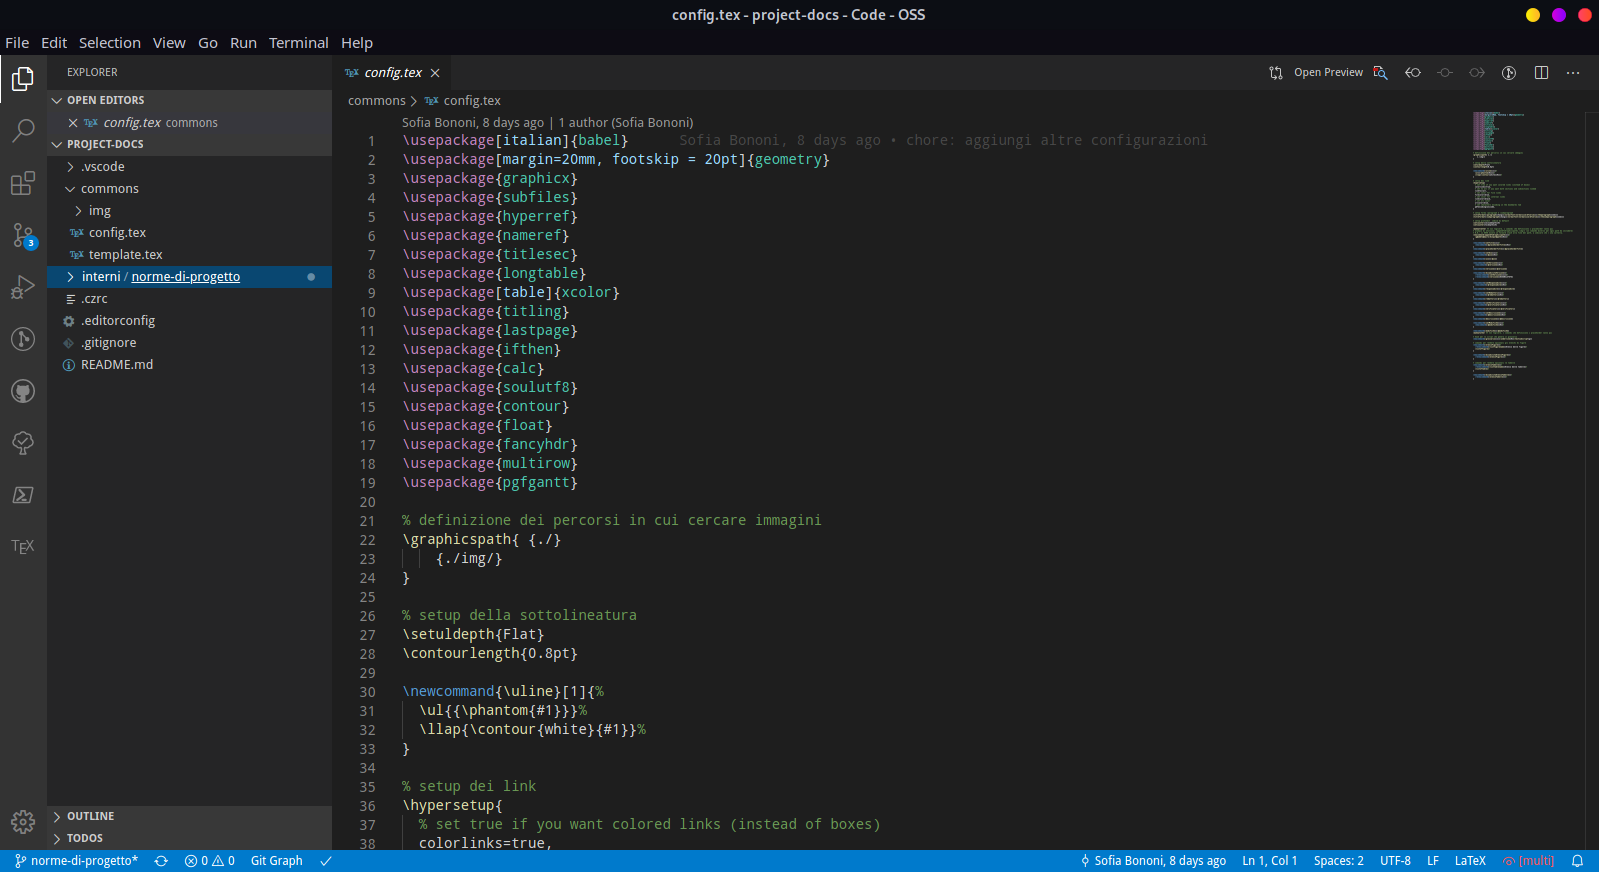
\includegraphics[width=10cm]{img/vscode.png}
  \label{fig:github}
  \caption{Visual Studio Code per GNU/Linux.}
\end{figure}

\subparagraph{Sistemi Operativi}
I sistemi operativi sui quali persistono gli strumenti software utilizzati sono:
\begin{itemize}
  \item Windows 10;
  \item macOS Catalina;
  \item Ubuntu 19.10;
  \item Debian 10;
  \item Manjaro Linux.
\end{itemize}

\end{document}
